\section{Entropy: Concept and Estimation}

\subsection{Noise}
\textbf{Noise} is any unwanted signal of random nature that modifies the intensity of the original signal to be perceived.

In the real world, signals are affected by uncontrollable elements that generate noise. This noise is typically superimposed as \textbf{additive noise}:

\begin{equation}
S(t) = f(t) + r(t)
\label{eq:additive_noise}
\end{equation}

where $S(t)$ is the received signal, $f(t)$ is the original signal, and $r(t)$ is the noise component.

The first stage in signal processing focuses on identifying and eliminating noisy artifacts, though complete elimination is usually not feasible. The random nature of noise means that signals with noise are not deterministic but rather \textbf{stochastic processes}, where repeated measurements of the same signal produce different results.

\subsubsection{Types of Noise}

\paragraph{Atmospheric Noise}
Atmospheric noise comes from electrical signals derived from natural discharges that occur under the ionosphere. Storms or electrical charges in clouds are sources of this type of noise, which generally affects communication systems using the radio spectrum more significantly. Approximately, the power of atmospheric noise is inversely proportional to frequency. Thus, atmospheric noise has greater impact on low and medium frequency bands, while lower power noise affects VHF and UHF bands. As a result, atmospheric noise affects AM communication bands and decreases significantly at TV and FM frequencies. Beyond 30 MHz, atmospheric noise has less negative impact than the receiver's own noise.

\paragraph{Man-Made Noise}
This refers to electrical artifacts generated by sources such as automobiles, electric motors, switches, high-voltage lines, etc. It is also known as \textbf{industrial noise}. The intensity of these noisy signals is greater in large urban centers and industrial areas. In these areas, noise of this nature prevails over other noise sources in the frequency range between 1 MHz and 600 MHz.

\paragraph{Impulsive or Shot Noise}
This type of noise causes the appearance of anomalous values (outliers) in the signal. It is characterized by a sudden increase in intensity during a short period of time. Generally, its origin is an external agent to the information system: a lightning strike or interference from a motor spark. However, it should not be confused with atmospheric or man-made noise, as the duration of these is more prolonged in time.

\paragraph{Galactic Noise}
It originates from disturbances produced beyond the Earth's atmosphere. The main sources of galactic noise are the sun and other stars.

\begin{itemize}
    \item \textbf{Solar}: The sun is a major source of energy emission in the form of electromagnetic radiation. These signals affect telecommunications systems. The frequency range of these emissions is very wide, including bands commonly used for radio communication systems. The intensity of the emission produced by the sun varies cyclically, with a period of approximately eleven years. At the highest levels, this radiation can make some frequency bands unusable.
    \item \textbf{Cosmic}: Like the sun, other stars near our planet emit energy in the form of electromagnetic radiation that can affect our signals and communication systems.
\end{itemize}

\paragraph{Thermal Noise}
This noise source is due to the random agitation of electrons in the elements of an electronic circuit. This movement could only be canceled under absolute zero temperature conditions. Therefore, it is an unavoidable noise source that will always be present in a signal acquisition and processing system. The movement of electrons increases as the temperature of the conductor increases, giving rise to small electrical currents. This noisy signal is distributed over a wide range of frequencies, so it will always affect the system to some degree, despite carrying out different filtering stages.

\paragraph{Flicker Noise or 1/f Noise}
It is called 1/f because its power decays below 1 kHz when frequency increases. Therefore, it has greater impact on low frequencies. The physical causes of this type of noise are not entirely clear. It originates in elements such as transistors or resistors, and it is hypothesized that it is due to intermodulation processes in these elements.

\subsubsection{Signal-to-Noise Ratio (SNR)}

When an information source is affected by noisy artifacts, the \textbf{Signal-to-Noise Ratio (SNR)} quantitatively indicates the quality of the signal of interest. This ratio is defined as the quotient between the power of the received signal and the estimated noise power. A value greater than unity (1) indicates a greater presence of the signal compared to the noise. The relationship between these power terms is generally expressed in decibels (dB).

\begin{equation}
\text{SNR} = 10\log_{10}\left(\frac{P_S}{P_N}\right)
\label{eq:snr}
\end{equation}

where:
\begin{itemize}
    \item $P_S$ corresponds to the signal power.
    \item $P_N$ corresponds to the noise power.
\end{itemize}

\paragraph{Example:}

Consider a communication system where the signal power is $P_S = 100$ and the noise power is $P_N = 10$. The SNR is calculated as:

\begin{align*}
\text{SNR} &= 10\log_{10}\left(\frac{P_S}{P_N}\right) \\
          &= 10\log_{10}\left(\frac{100}{10}\right) \\
          &= 10\log_{10}(10) \\
          &= 10 \times 1 = 10 \text{ dB}
\end{align*}

This means the signal power is 10 times greater than the noise power (a ratio of 10:1), resulting in an SNR of 10 dB.

\textbf{Interpretation of SNR values:}
\begin{itemize}
    \item \textbf{SNR greater than 0 dB}: Signal power exceeds noise power (good quality)
    \item \textbf{SNR = 0 dB}: Signal and noise powers are equal
    \item \textbf{SNR lower than 0 dB}: Noise power exceeds signal power (poor quality)
    \item \textbf{SNR = 20 dB}: Signal is 100 times stronger than noise (excellent quality)
    \item \textbf{SNR = 3 dB}: Signal is approximately 2 times stronger than noise (minimum acceptable for many applications)
\end{itemize}

\subsection{Entropy}
Signals contain information and are affected by various noise sources. In this context, the concept of \textbf{entropy} arises. Similar to physics, the term refers to the complexity of the signal. The addition of noise increases the degree of complexity of a signal, resulting in higher entropy.

In information theory, \textbf{entropy} is defined as the amount of information from a random source (on average). Therefore, entropy serves to \textbf{characterize a random variable}. Signals can be modeled as a sequence of realizations of a random variable over time (stochastic process), so we will see how to extend the definition of entropy to random elements of this nature.

\subsubsection{Shannon's Entropy Definition}

Given a discrete random variable $X$ that takes values from the set $\{x_1, x_2, \ldots, x_M\}$ with probability distribution $P(X = x_i) = p_i$, Shannon defined entropy as:

\begin{equation}
H(X) = E\{-\log_2[P(X)]\} = \sum_{i=1}^{M} -\log_2[P(x_i)] \cdot P(x_i) = \sum_{i=1}^{M} -p_i \log_2(p_i)
\label{eq:shannon_entropy}
\end{equation}

where $-\log_2[P(x_i)]$ is interpreted as the \textbf{quantity of information} (or \textbf{self-information}) associated with outcome $x_i$.

\begin{tcolorbox}[colback=blue!5!white, colframe=blue!75!black, title=\textbf{Curious Fact: What Does $E$ Mean?}]
The capital $E$ denotes the \textbf{expected value} (also called expectation or mean). For a discrete random variable, the expected value of a function $g(X)$ is calculated as:
\begin{equation}
E[g(X)] = \sum_{i=1}^{M} g(x_i) \cdot P(x_i)
\end{equation}
In the entropy formula, $E\{-\log_2[P(X)]\}$ means we take the expected value of the information content $-\log_2[P(X)]$, which gives us the average information across all possible outcomes.
\end{tcolorbox}

\subsubsection{Understanding the Formula}

The key insight is that \textbf{less probable values carry more information} (surprise effect) compared to more probable values. For example:
\begin{itemize}
    \item If an event is very likely ($p_i \approx 1$), then $-\log_2(p_i) \approx 0$: we learn little new information.
    \item If an event is very unlikely ($p_i \approx 0$), then $-\log_2(p_i)$ is large: we learn a lot of new information.
\end{itemize}

Entropy $H(X)$ is the \textbf{expected value} (average) of this information content across all possible outcomes.

\subsubsection{Example: Bernoulli Distribution}

Consider a random variable $X$ with only two possible outcomes, $\{x_1, x_2\}$ (a \textbf{Bernoulli distribution}). Let $P(X = x_1) = p$ and $P(X = x_2) = 1-p$. The entropy is:

\begin{equation}
H(X) = -p \log_2(p) - (1-p) \log_2(1-p)
\label{eq:bernoulli_entropy}
\end{equation}

The entropy reaches its \textbf{maximum value of 1} when $p = 0.5$. In this case, both events have equal probability, and on average we obtain the same amount of information from $X$. When $p$ approaches 0 or 1, the entropy approaches 0, meaning we can almost predict the outcome with certainty, so we learn little new information.

\textbf{Concrete Example:} Consider a fair coin flip where $p = 0.5$:
\begin{align*}
H(X) &= -0.5 \log_2(0.5) - 0.5 \log_2(0.5) \\
     &= -0.5 \cdot (-1) - 0.5 \cdot (-1) \\
     &= 0.5 + 0.5 = 1
\end{align*}
This means each coin flip provides an entropy of 1 on average. If the coin is biased (e.g., $p = 0.9$ for heads), then:
\begin{align*}
H(X) &= -0.9 \log_2(0.9) - 0.1 \log_2(0.1) \\
     &\approx 0.469
\end{align*}
The entropy is lower because we can predict the outcome more easily (heads is very likely), so we learn less information.

Figure~\ref{fig:bernoulli_entropy} shows the variation of entropy $H(X)$ as a function of the probability $P(X = x_1) = p$ for a Bernoulli distribution. The curve is symmetric and reaches its maximum value of 1 when $p = 0.5$, demonstrating that uncertainty (entropy) is highest when both outcomes are equally probable.

\begin{figure}[H]
    \centering
    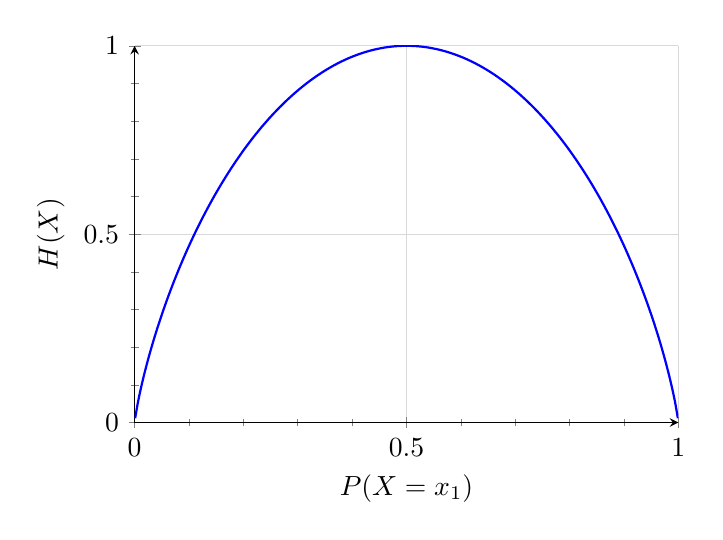
\begin{tikzpicture}
        \begin{axis}[
            width=0.7\textwidth,
            height=0.525\textwidth,
            xlabel={$P(X = x_1)$},
            ylabel={$H(X)$},
            xmin=0, xmax=1,
            ymin=0, ymax=1,
            grid=major,
            grid style={gray!30},
            axis lines=left,
            xtick={0, 0.5, 1},
            ytick={0, 0.5, 1},
            minor xtick={0.1,0.2,0.3,0.4,0.6,0.7,0.8,0.9},
            minor ytick={0.1,0.2,0.3,0.4,0.6,0.7,0.8,0.9},
            minor grid style={gray!10},
            legend pos=north east,
        ]
        \addplot[
            domain=0.001:0.999,
            samples=200,
            smooth,
            thick,
            blue,
        ] {-x*log2(x) - (1-x)*log2(1-x)};
        \end{axis}
    \end{tikzpicture}
    \caption{Entropy $H(X)$ as a function of probability $P(X = x_1) = p$ for a Bernoulli distribution. The entropy reaches its maximum value of 1 when $p = 0.5$ (equal probability for both outcomes) and approaches 0 when $p$ approaches 0 or 1 (certain outcomes).}
    \label{fig:bernoulli_entropy}
\end{figure}

\subsection{Signals as Stochastic Processes}

Signals can be modeled mathematically as a set of random variables (a \textbf{stochastic process}). For example, a voice signal of a certain duration can be viewed as a finite time series, where each sample represents a realization of a random variable.

Including new samples in the series increases the information content, showing that process entropy depends on its length. Therefore, it makes sense to measure the variation of signal entropy due to the inclusion of a new sample. This is called the \textbf{entropy rate} or \textbf{differential entropy}.

\subsubsection{Entropy of a Stochastic Process}

Consider a signal of length $N$ as a sequence of $N$ random variable realizations: $\mathbf{x} = x_1, x_2, \ldots, x_N$. Figure~\ref{fig:signal_sequence} illustrates this concept, showing a signal where each sample $x_i$ represents a realization of a random variable at time index $i$.

\begin{figure}[H]
    \centering
    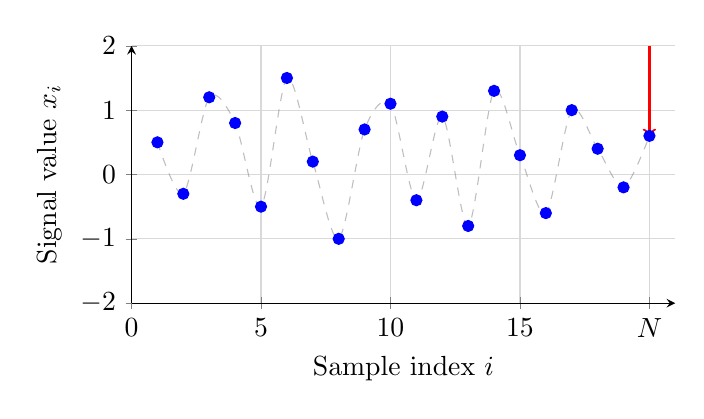
\begin{tikzpicture}
        \begin{axis}[
            width=0.7\textwidth,
            height=0.4\textwidth,
            xlabel={Sample index $i$},
            ylabel={Signal value $x_i$},
            xmin=0, xmax=21,
            ymin=-2, ymax=2,
            grid=major,
            grid style={gray!30},
            axis lines=left,
            xtick={0,5,10,15,20},
            xticklabels={0,5,10,15,$N$},
            ytick={-2,-1,0,1,2},
        ]
        % Generate some random-looking signal values
        \addplot[
            only marks,
            mark=*,
            mark size=2pt,
            blue,
        ] coordinates {
            (1,0.5) (2,-0.3) (3,1.2) (4,0.8) (5,-0.5)
            (6,1.5) (7,0.2) (8,-1.0) (9,0.7) (10,1.1)
            (11,-0.4) (12,0.9) (13,-0.8) (14,1.3) (15,0.3)
            (16,-0.6) (17,1.0) (18,0.4) (19,-0.2) (20,0.6)
        };
        \addplot[
            smooth,
            dashed,
            gray,
            opacity=0.5,
        ] coordinates {
            (1,0.5) (2,-0.3) (3,1.2) (4,0.8) (5,-0.5)
            (6,1.5) (7,0.2) (8,-1.0) (9,0.7) (10,1.1)
            (11,-0.4) (12,0.9) (13,-0.8) (14,1.3) (15,0.3)
            (16,-0.6) (17,1.0) (18,0.4) (19,-0.2) (20,0.6)
        };
        % Add annotation for N
        \node[above] at (axis cs:20,2.2) {$N=20$};
        \draw[->, red, thick] (axis cs:20,2.0) -- (axis cs:20,0.6);
        \end{axis}
    \end{tikzpicture}
    \caption{A signal of length $N=20$ as a sequence of random variable realizations. Each point $(i, x_i)$ represents a sample where $i$ is the time index and $x_i$ is the realization of the random variable at that time.}
    \label{fig:signal_sequence}
\end{figure}

The entropy $H_N$ of this stochastic process is:

\begin{equation}
\begin{split}
H_N &= E\{-\log_2[p(x_1, x_2, \ldots, x_N)]\} \\
&= -\int_{-\infty}^{\infty} \log_2[p(x_1, x_2, \ldots, x_N)] \cdot p(x_1, x_2, \ldots, x_N) \, dx_1 \ldots dx_N
\end{split}
\label{eq:stochastic_entropy}
\end{equation}

where $p(x_1, x_2, \ldots, x_N)$ is the joint probability density function (PDF) of the variables composing the stochastic process.

\begin{tcolorbox}[colback=blue!5!white, colframe=blue!75!black, title=\textbf{Note: Computational Complexity}]
Computing entropy using the stochastic process formula is \textbf{much more computationally expensive} than ApEn:

\begin{itemize}
    \item \textbf{Stochastic process entropy}: Requires estimating an $N$-dimensional joint PDF and computing an $N$-dimensional integral. The complexity grows exponentially with $N$ (curse of dimensionality), making it impractical for long signals.
    \item \textbf{ApEn}: Works with fixed-length subseries ($m$ is typically 2-3), requiring only pattern matching. Complexity is approximately $O(N^2)$, which is manageable even for long signals.
\end{itemize}

This computational advantage is one of the main reasons why ApEn is widely used in practice.
\end{tcolorbox}

\subsubsection{Entropy Rate}

The \textbf{entropy rate} $E_N$ of the signal is defined as:

\begin{equation}
E_N = \lim_{N \to \infty} (H_{N+1} - H_N)
\label{eq:entropy_rate}
\end{equation}

This represents the change in entropy when a new sample is added to an infinitely long sequence.

\begin{tcolorbox}[colback=blue!5!white, colframe=blue!75!black, title=\textbf{Note}]
The entropy rate measures how much entropy increases (on average) when you add one more sample to a long signal.
\end{tcolorbox}

\subsubsection{Approximate Entropy (ApEn)}

There are various methods for estimating signal entropy. \textbf{Approximate Entropy (ApEn)} is one such estimation procedure. The algorithm involves estimating the entropy of subseries of length $m$ and $m+1$. The final entropy value is obtained by taking the difference between these two estimations.

\paragraph{Methodology:}

Consider an original time series $\mathbf{x} = [x_1, x_2, \ldots, x_N]$.

\textbf{Step 1: Extract subseries.} Extract all subseries of length $m$, denoted as $x_i^{(m)} = [x_i, x_{i+1}, \ldots, x_{i+m-1}]$ for $i = 1, 2, \ldots, N-m+1$.

\textbf{Step 2: Find similar subseries.} Given a tolerance $r$, count the number of subseries $N^{(m)}(i)$ that are similar to $x_i^{(m)}$, where similarity is determined by a distance metric $d[x_i^{(m)}, x_j^{(m)}] \leq r$.

\textbf{Step 3: Calculate probability.} The probability of finding a subseries similar to $x_i^{(m)}$ in the original series is:
\begin{equation}
C^{(m)}(i) = \frac{N^{(m)}(i)}{N - m + 1}
\label{eq:apen_probability}
\end{equation}
where $N - m + 1$ is the total number of subseries of length $m$ that can be extracted from the original series.

\textbf{Step 4: Estimate entropy.} The term $C^{(m)}(i)$ provides a discrete estimation of the probability density function. Using Shannon's entropy definition, the entropy of the process represented by $x^{(m)}$ is:
\begin{equation}
H_N^{(m)} = -\frac{1}{N - m + 1} \sum_{i=1}^{N-m+1} \log_2[C^{(m)}(i)]
\label{eq:apen_entropy}
\end{equation}

The Approximate Entropy is then calculated as:
\begin{equation}
\text{ApEn}(m, r, N) = H_N^{(m)} - H_N^{(m+1)}
\label{eq:apen}
\end{equation}

\begin{tcolorbox}[colback=blue!5!white, colframe=blue!75!black, title=\textbf{Note: ApEn vs. Entropy Rate}]
Approximate Entropy (ApEn) is \textbf{not exactly the same} as the entropy rate, but they are related concepts:

\begin{itemize}
    \item \textbf{Entropy rate} $E_N = \lim_{N \to \infty} (H_{N+1} - H_N)$ measures the change in entropy when adding one more \textbf{sample} to the sequence.
    \item \textbf{ApEn} $= H_N^{(m)} - H_N^{(m+1)}$ measures the change in entropy when increasing the \textbf{subseries length} from $m$ to $m+1$.
\end{itemize}

ApEn is an \textbf{approximation} of the entropy rate. Instead of computing the theoretical entropy rate (which requires the full joint PDF), ApEn estimates it by analyzing patterns in subseries of different lengths. Both measure how entropy changes with sequence length, but ApEn uses a practical, pattern-based approach rather than the theoretical limit.
\end{tcolorbox}

\paragraph{Example:}

Consider a time series $\mathbf{x} = [1.0, 1.2, 0.9, 1.1, 1.3, 0.8]$ with $N = 6$. Let $m = 2$ and $r = 0.2$.

\textbf{Step 1: Extract subseries of length $m = 2$:}
\begin{itemize}
    \item $x_1^{(2)} = [1.0, 1.2]$
    \item $x_2^{(2)} = [1.2, 0.9]$
    \item $x_3^{(2)} = [0.9, 1.1]$
    \item $x_4^{(2)} = [1.1, 1.3]$
    \item $x_5^{(2)} = [1.3, 0.8]$
\end{itemize}

\textbf{Step 2: Find similar subseries.} Using the Chebyshev distance (maximum absolute difference between corresponding elements), we count how many subseries are within tolerance $r = 0.2$ of each $x_i^{(2)}$. Two subseries are similar if $d[x_i^{(m)}, x_j^{(m)}] = \max_k |x_{i+k} - x_{j+k}| \leq r$.

For example, comparing $x_1^{(2)} = [1.0, 1.2]$ with $x_4^{(2)} = [1.1, 1.3]$:
\begin{align*}
d[x_1^{(2)}, x_4^{(2)}] &= \max(|1.0 - 1.1|, |1.2 - 1.3|) \\
                         &= \max(0.1, 0.1) = 0.1 \leq 0.2
\end{align*}
Since $0.1 \leq 0.2$, these subseries are similar.

Results for all subseries:
\begin{itemize}
    \item For $x_1^{(2)} = [1.0, 1.2]$: $N^{(2)}(1) = 2$ (matches itself and $x_4^{(2)} = [1.1, 1.3]$)
    \item For $x_2^{(2)} = [1.2, 0.9]$: $N^{(2)}(2) = 1$ (only itself)
    \item For $x_3^{(2)} = [0.9, 1.1]$: $N^{(2)}(3) = 1$ (only itself)
    \item For $x_4^{(2)} = [1.1, 1.3]$: $N^{(2)}(4) = 2$ (matches itself and $x_1^{(2)}$)
    \item For $x_5^{(2)} = [1.3, 0.8]$: $N^{(2)}(5) = 1$ (only itself)
\end{itemize}

\textbf{Step 3: Calculate probabilities.} With $N - m + 1 = 6 - 2 + 1 = 5$ total subseries:
\begin{align*}
C^{(2)}(1) &= \frac{2}{5} = 0.4 \\
C^{(2)}(2) &= \frac{1}{5} = 0.2 \\
C^{(2)}(3) &= \frac{1}{5} = 0.2 \\
C^{(2)}(4) &= \frac{2}{5} = 0.4 \\
C^{(2)}(5) &= \frac{1}{5} = 0.2
\end{align*}

\textbf{Step 4: Estimate entropy.}
\begin{align*}
H_6^{(2)} &= -\frac{1}{5} \sum_{i=1}^{5} \log_2[C^{(2)}(i)] \\
          &= -\frac{1}{5}[\log_2(0.4) + \log_2(0.2) + \log_2(0.2) + \log_2(0.4) + \log_2(0.2)] \\
          &\approx -\frac{1}{5}[-1.32 - 2.32 - 2.32 - 1.32 - 2.32] \\
          &\approx 1.92
\end{align*}

Similarly, we would compute $H_6^{(3)}$ for subseries of length $m+1 = 3$, and then:
$$\text{ApEn}(2, 0.2, 6) = H_6^{(2)} - H_6^{(3)}$$

\begin{tcolorbox}[colback=yellow!5!white, colframe=yellow!75!black, title=\textbf{Takeaway: Why is ApEn Useful?}]
Approximate Entropy is a practical and powerful tool for signal analysis because:

\begin{itemize}
    \item \textbf{Practical estimation}: It provides a computationally feasible way to estimate entropy without requiring knowledge of the full probability distribution, making it applicable to real-world signals.
    \item \textbf{Pattern detection}: By analyzing subseries patterns, ApEn can detect regularity and predictability in signals, which is useful for characterizing signal complexity.
    \item \textbf{Noise robustness}: The tolerance parameter $r$ allows ApEn to be robust to noise, focusing on overall patterns rather than exact matches.
    \item \textbf{Wide applications}: ApEn is widely used in biomedical signal processing (EEG, ECG), time series analysis, and any domain where quantifying signal complexity or regularity is important.
    \item \textbf{Comparative analysis}: It enables comparison of entropy between different signals or different segments of the same signal, helping identify changes in signal characteristics.
\end{itemize}
\end{tcolorbox}

\subsection{Entropy in Images}

The entropy value of a signal can be interpreted as its degree of uncertainty. Equivalently, it reflects the capacity to predict a future state or value from the knowledge or observation of previous signal values. A higher entropy value reflects greater complexity and chaos in the signal under study.

As a result, entropy gives us an idea of the level of noise impact on a signal. If we take a sample of the same signal under the same conditions but at different time instants, the signal with higher entropy will be the one with a higher noise level.

\subsubsection{Images vs. One-Dimensional Signals}

The nature and mathematical modeling of images are different from one-dimensional time-dependent signals. An image does not have an implicit time variable, as occurs in a voice signal or an electrocardiogram, but rather represents light captured at each spatial position. Additionally, image information is represented in two dimensions.

Therefore, in images, just as in time series we characterized the rate of entropy increase with respect to new samples, we could think of an entropy rate with respect to the unit area represented. For entropy estimation in an image, the histogram of intensity levels is used. The final estimation is obtained as the entropy of the random variable characterized by this histogram.

As with one-dimensional signals, entropy will tend to increase, or at least remain the same, if the image area considered for estimation is enlarged. Thus, lower entropy values will be associated with repetitive patterns in the image that lead to a histogram with marked peaks (texture). In contrast, entropy increases if there is greater variability in the intensity values observed in the image, with no marked patterns producing a flatter histogram. In this sense, it follows that noise contributes to increasing the entropy of the image, as it causes the variability of the observed intensity levels to increase.

\subsection{Mathematical Characterization of Noise: Stochastic Processes}

The term \textbf{stochastic process} has been previously used in this topic to refer to a random signal. In our case, any signal will be the result of the combination of the signal of interest and an unwanted signal, of random and chaotic nature, which contributes to increasing entropy. This unwanted signal is noise.

Therefore, the resulting signal is, in itself, a random signal. Just as happens with a random variable, from which we take a sample and obtain values according to a probability density function, the signals we handle are realizations of a stochastic process. Each time we extract a sample from the information source, we obtain a different signal.

In this section, a formal definition of stochastic process is provided that allows understanding the modeling and characterization of noise in signal processing.

\subsubsection{Random Variables}

A random variable is characterized by the following three elements:

\begin{itemize}
    \item \textbf{Sample space}: The set of all possible outcomes that can be observed in the realization of an experiment.
    \item \textbf{Set of events}: Subset of the sample space.
    \item \textbf{Probability law}: Assignment of probability to each of the observable events.
\end{itemize}

\paragraph{Example: Rolling a Fair Die}

Consider the experiment of rolling a fair six-sided die:

\begin{itemize}
    \item \textbf{Sample space}: $\Omega = \{1, 2, 3, 4, 5, 6\}$ (all possible outcomes)
    \item \textbf{Set of events}: Examples include:
    \begin{itemize}
        \item Event $A$: "Rolling an even number" = $\{2, 4, 6\}$
        \item Event $B$: "Rolling a number greater than 4" = $\{5, 6\}$
        \item Event $C$: "Rolling a 3" = $\{3\}$
    \end{itemize}
    \item \textbf{Probability law}: For a fair die, each outcome has equal probability:
    \begin{itemize}
        \item $P(1) = P(2) = P(3) = P(4) = P(5) = P(6) = \frac{1}{6}$
        \item $P(A) = P(\{2, 4, 6\}) = \frac{3}{6} = \frac{1}{2}$
        \item $P(B) = P(\{5, 6\}) = \frac{2}{6} = \frac{1}{3}$
    \end{itemize}
\end{itemize}

\paragraph{Example: Signal Intensity Measurement}

In signal processing, consider measuring the intensity of a signal at a specific time:

\begin{itemize}
    \item \textbf{Sample space}: $\Omega = [0, 255]$ (all possible intensity values, e.g., for an 8-bit image)
    \item \textbf{Set of events}: Examples include:
    \begin{itemize}
        \item Event $D$: "Intensity between 100 and 150" = $[100, 150]$
        \item Event $E$: "Intensity greater than 200" = $(200, 255]$
    \end{itemize}
    \item \textbf{Probability law}: Defined by a probability density function (PDF) $f(x)$ that assigns probabilities to intervals, such as:
    \begin{itemize}
        \item $P(D) = \int_{100}^{150} f(x) \, dx$
        \item $P(E) = \int_{200}^{255} f(x) \, dx$
    \end{itemize}
\end{itemize}

\subsubsection{Stochastic Processes}

A stochastic process can be viewed as a random variable for which the result of an experiment is given in the form of a signal. In the same way as a random variable, it is characterized by the three elements mentioned: sample space, set of events, and probability assignment law.

In practice, as previously mentioned in this topic, we will have noisy signals that, from a mathematical point of view, will be modeled as a stochastic process. The noise component will be assumed to be additive, so the captured signal will have the following form:

\begin{equation}
y(t) = x(t) + \varepsilon(t)
\label{eq:noisy_signal}
\end{equation}

where:
\begin{itemize}
    \item $x(t)$ reflects the signal of interest.
    \item $\varepsilon(t)$ corresponds to the noise.
\end{itemize}

\paragraph{Example: Sinusoidal Signal with Gaussian Noise}

Consider, for example, that the signal of interest corresponds to a tone of frequency $f$ and that the noise component follows a Gaussian distribution with zero mean and variance $\sigma^2$.

In Figure~\ref{fig:stochastic_signal}, we can see this target signal (top) and a realization of the stochastic process that corresponds to the observed signal (bottom).

\begin{figure}[H]
    \centering
    \includegraphics[width=0.7\textwidth]{img/stocastic_001.png}
    \caption{Comparison of a clean sinusoidal signal (top) and a noisy realization of the stochastic process (bottom). The noise component gives the signal a random nature that prevents us from knowing its exact value at any instant $t$.}
    \label{fig:stochastic_signal}
\end{figure}

As can be seen, the noise component gives the signal a random nature that prevents us from knowing its exact value at any instant $t$. In order to characterize the stochastic process, the objective will be to know its statistical properties. Probability distribution and density functions allow us to model the process statistically.

These functions are given as follows:

\begin{itemize}
    \item \textbf{Distribution function}: $F_X(x,t) = P(X(t) \leq x)$
    \item \textbf{Probability density function}: $f_X(x,t) = \frac{dF_X(x,t)}{dx}$
\end{itemize}

From these functions, the stationarity of the process can be defined:

\begin{itemize}
    \item A process is stationary in \textbf{strict sense} if the probability density function that characterizes the process does not vary with time. That is, for a constant $c$ such that $c > 0$, the following will hold: $f_X(x,t) = f_X(x,t+c)$
    \item A process is stationary in \textbf{wide sense} if the statistical moments that characterize it (mean, variance, etc.) do not vary with respect to time.
\end{itemize}

\paragraph{Example: Strict-Sense Stationarity}

Consider a process $X(t) = A \sin(2\pi f t + \phi)$, where $A$ and $\phi$ are random variables, and $f$ is a constant frequency. If $A$ and $\phi$ are independent, with $A$ having a fixed distribution and $\phi$ uniformly distributed on $[0, 2\pi]$, then the PDF of $X(t)$ at any time $t$ is the same (it depends only on the distribution of $A$ and $\phi$, not on $t$). This process is stationary in strict sense because $f_X(x,t) = f_X(x,t+c)$ for any $c$.

\paragraph{Example: Wide-Sense Stationarity}

Consider white noise $\varepsilon(t)$ with zero mean and constant variance $\sigma^2$:
\begin{itemize}
    \item Mean: $E[\varepsilon(t)] = 0$ (constant, independent of $t$)
    \item Variance: $\text{Var}[\varepsilon(t)] = \sigma^2$ (constant, independent of $t$)
    \item Autocorrelation: $E[\varepsilon(t)\varepsilon(t+\tau)] = \sigma^2 \delta(\tau)$ (depends only on $\tau$, not on $t$)
\end{itemize}
This process is stationary in wide sense because its statistical moments (mean and variance) do not vary with time, even though we may not know the full PDF.

\paragraph{Example: Non-Stationary Process}

Consider a process $Y(t) = t + \varepsilon(t)$, where $\varepsilon(t)$ is white noise. The mean of this process is $E[Y(t)] = t$, which clearly varies with time. Therefore, this process is \textbf{not stationary} (neither in strict sense nor in wide sense) because its statistical properties change over time.

\paragraph{Example: Non-Stationary Signal with Trend}

Let us return to the previous example. In this case, the captured signal shows, in addition to Gaussian noise, another component that causes a clear trend over time. Figure~\ref{fig:nonstationary_trend} shows this new example.

\begin{figure}[H]
    \centering
    \includegraphics[width=0.7\textwidth]{img/stochastic_002.png}
    \caption{Non-stationary signal with a trend component. The signal exhibits both Gaussian noise and a clear trend over time, making its statistical properties vary along the temporal axis.}
    \label{fig:nonstationary_trend}
\end{figure}

As a result of this trend, the statistical properties of the signal do not remain constant along the temporal axis, so it cannot be considered a stationary signal. It will be necessary to eliminate the noise component that causes this trend to remove the non-stationarity present in our information.
